%%%%%%%%%%%%%%%%%%%%%%%%%%%%% DEFAULT TEXT FILE %%%%%%%%%%%%%%%%%%%%%%%%%%%%%
\documentclass[12pt,a4paper]{article}
\usepackage[utf8]{inputenc}             % Default unicode
\usepackage{hyperref}
\usepackage{multicol}
\usepackage{geometry}
\usepackage{graphicx}                      % images
\usepackage{fontawesome}     %\faicon      % icons
\usepackage{pifont}    %\ding{118}         % symbols
\usepackage{tikz}                           % graphics
\usepackage{listings,xcolor}
\usepackage{fancyhdr}
\usepackage[edges]{forest}

\tolerance=1
\emergencystretch=\maxdimen
\hyphenpenalty=10000
\hbadness=10000
\renewcommand{\indent}{\hspace\parindent}
\geometry{headheight=16pt, margin=1in}
\graphicspath{ {../screenshots} }

%%%%%%%%%%%%%%%%%%%%%%%%%%%%%%%% PROGRAMMING %%%%%%%%%%%%%%%%%%%%%%%%%%%%%%%%
\definecolor{backcolour}{rgb}{0.96,0.96,0.96}
\definecolor{dkgreen}{rgb}{0,0.6,0}
\definecolor{gray}{rgb}{0.5,0.5,0.5}
\definecolor{mauve}{rgb}{0.58,0,0.82}
\definecolor{darkerblue}{HTML}{010161}
\definecolor{foldercolor}{RGB}{124,166,198}

\lstset{
    language=Python,
    showstringspaces=false,
    columns=flexible,
    basicstyle=\ttfamily\footnotesize,
    numbers=none,                    
    backgroundcolor=\color{backcolour},   
    numberstyle=\tiny\color{gray},
    keywordstyle=\color{blue},
    commentstyle=\color{dkgreen},
    stringstyle=\color{mauve},
    keepspaces=false,                 
    numbersep=5pt,                  
    showspaces=false,                
    showstringspaces=false,
    breaklines=true,
    breakatwhitespace=false,
    tabsize=2,
    postbreak=\mbox{\textcolor{red}{$\hookrightarrow$}\space}
}

\pagestyle{fancy}
\fancyhf{}
\fancyhead[L]{\color{darkerblue} Discrete Structures II}
\fancyhead[R]{\color{darkerblue} Invento Documentation $\|$ \partname{} \thepart{}}
\fancyfoot[C]{\thepage}
\renewcommand{\headrulewidth}{0pt}


\tikzset{pics/folder/.style={code={%
    \node[inner sep=0pt, minimum size=#1](-foldericon){};
    \node[folder style, inner sep=0pt, minimum width=0.3*#1, minimum height=0.6*#1, above right, xshift=0.05*#1] at (-foldericon.west){};
    \node[folder style, inner sep=0pt, minimum size=#1] at (-foldericon.center){};}
    },
    pics/folder/.default={20pt},
    folder style/.style={draw=foldercolor!80!black,top color=foldercolor!40,bottom color=foldercolor}
}

\forestset{is file/.style={edge path'/.expanded={%
        ([xshift=\forestregister{folder indent}]!u.parent anchor) |- (.child anchor)},
        inner sep=1pt},
    this folder size/.style={edge path'/.expanded={%
        ([xshift=\forestregister{folder indent}]!u.parent anchor) |- (.child anchor) pic[solid]{folder=#1}}, inner ysep=0.6*#1},
    folder tree indent/.style={before computing xy={l=#1}},
    folder icons/.style={folder, this folder size=#1, folder tree indent=3*#1},
    folder icons/.default={12pt},
}

%%%%%%%%%%%%%%%%%%%%%%%%% TABLE OF CONTENTS SETTINGS %%%%%%%%%%%%%%%%%%%%%%%%
\renewcommand{\contentsname}{\Huge\bfseries Table of Contents}

%%%%%%%%%%%%%%%%%%%%%%%%%%%%%%%%%%%%%%%%%%%%%%%%%%%%%%%%%%%%%%%%%%%%%%%%%%%%%
%%%%%%%%%%%%%%%%%%%%%%%%%%%%%%%%%% DOCUMENT %%%%%%%%%%%%%%%%%%%%%%%%%%%%%%%%%
\begin{document}
%%%%%%%%%%%%%%%%%%%%%%%%%%%%%%%%%%% TITLE %%%%%%%%%%%%%%%%%%%%%%%%%%%%%%%%%%%
    \thispagestyle{empty}
    \pagenumbering{roman}
    \addcontentsline{toc}{section}{Title page}

    \vspace*{\fill}
    \begingroup
    \centering

        \textbf{POLYTECHNIC UNIVERSITY OF THE PHILIPPINES\\
        BACHELOR OF SCIENCE IN COMPUTER SCIENCE}\vspace{.1in}

        \noindent
\includegraphics[width=3in,height=3in]{logo.png}\vspace{.1in}

        \textbf{DISCRETE STRUCTURES II}\vspace{.1in}
        
        \textbf{\huge Invento Management System Documentation}\vspace{2in}

    \endgroup
    \vspace*{\fill}

        \noindent\textbf{BSCS 2-1N\\Group 3}\vspace{0.2in}

        \noindent
        \begin{tabular}{l l}
            \textbf{Project Manager:} & Annalyn Belen \\
            \textbf{Designer:} & Monika Jea Ng\\
            \textbf{Developer:} & Steve Pabular \\
            \textbf{Systems Analyst:} & John Nicolas Oandasan\\
            \textbf{Business Analyst:} & Hazel Conception\\
            \textbf{Technical Writer:} & Percian Cayaban
        \end{tabular}\vspace{0.2in}

        \noindent\textbf{Instructor:} Prof. Angie Payne

    %%%%%%%%%%%%%%%%%%%%%%%%%%%%% TABLE OF CONTENTS %%%%%%%%%%%%%%%%%%%%%%%%%%%%%
    \newpage
    \thispagestyle{plain}
    \addcontentsline{toc}{section}{Contents}
    \tableofcontents

    %%%%%%%%%%%%%%%%%%%%%%%%%%%%%%%%%% CONTENT %%%%%%%%%%%%%%%%%%%%%%%%%%%%%%%%%%
    \newpage
    \pagenumbering{arabic}
    \setcounter{page}{1}
    \part{ Invento Management System }

    \section*{Overview \hrulefill}
        \addcontentsline{toc}{section}{Overview}
        \indent
        \texttt{Invento} is an inventory management system that allows users to 
        manage their inventory of products, track sales, and view sales data in 
        real-time. The system supports multiple user roles, including \texttt{Admin} 
        and \texttt{User} accounts, and provides other variety of features.

        \noindent\hrulefill

    \section*{Features}
        \addcontentsline{toc}{section}{Features}

        \begin{enumerate}
            \item{\textbf{Login and Registration}} - To access the system, users must 
                first register an account or log in with an existing account. This 
                feature allows tracking whose changes were implemented in the 
                inventory. This also saves the current session for future access.
            \item{\textbf{Admin and User Accounts}} - Users can control the inventory 
                and sales data. Administrators had access to additional features, 
                including the ability to reset inventory, delete accounts, and manage 
                user accounts.
            \item{\textbf{Sales Graph}} - Displays a line graph of sales data for the 
                past 7 days. The graph updates in real-time as new sales data is 
                entered into the system.
            \item{\textbf{Product Management}} - Users and admins can add, edit, and 
                remove products from the inventory. Changes can be seen in the table 
                displayed.
            \item{\textbf{Account Settings}} - Users and admin can change their 
                passwords and display pictures. They could also personalize the 
                themes of the program in settings.
        \end{enumerate}
        

    \section*{Setup}
        \addcontentsline{toc}{section}{Setup}

        This program requires the 3.10+ version of Python installed and the 
        following packages:

        \begin{itemize}
            \item \texttt{customtkinter}
            \item \texttt{Pillow}
            \item \texttt{matplotlib}
        \end{itemize}

        \noindent Which can be installed with the following command:

        \hfill{}

        \texttt{pip install --upgrade customtkinter Pillow matplotlib}

        \hfill{}

        \noindent There also is a detailed setup guide available at 
        \href{https://github.com/steguiosaur/invento}{\textcolor{blue}
        {https://github.com/steguiosaur/invento}}.


    \newpage
    \part{User Guide}

        \indent The program can be executed by using the command \texttt{python Main.py} in a terminal. If there aren't any dependency 
        conflicts and logged-in session, it will show the Login page 
        (Figure \ref{fig:login}) wherein it takes an input for the current 
        registered accounts.

        \begin{figure}[ht]
          \centering
          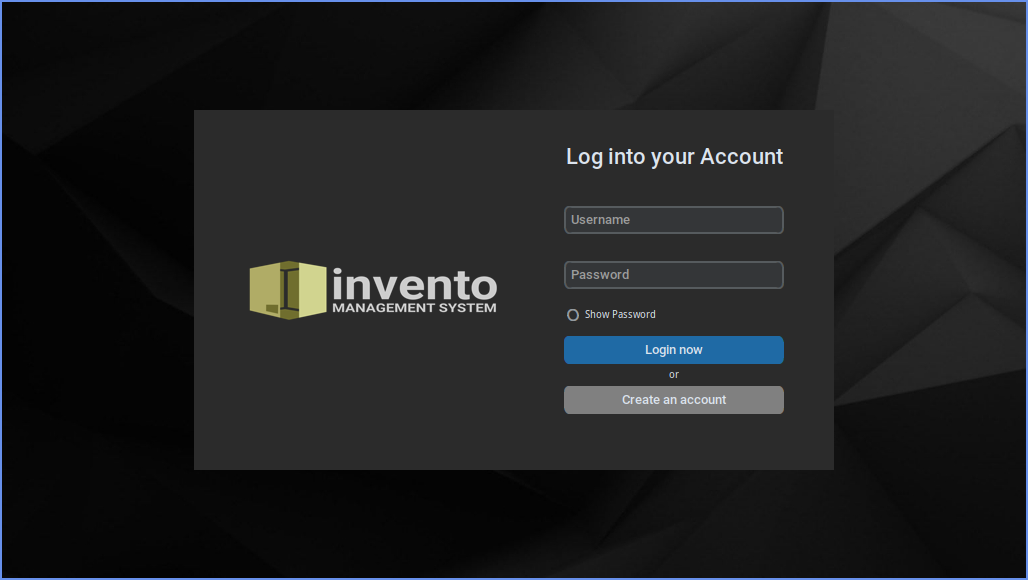
\includegraphics[width=5in,height=3in]{Login.png}
          \caption{Login page}
          \label{fig:login}
        \end{figure}

        \indent
        On this page (Figure \ref{fig:register}), you could register a new 
        account by entering the required information.

        \begin{figure}[ht]
          \centering
          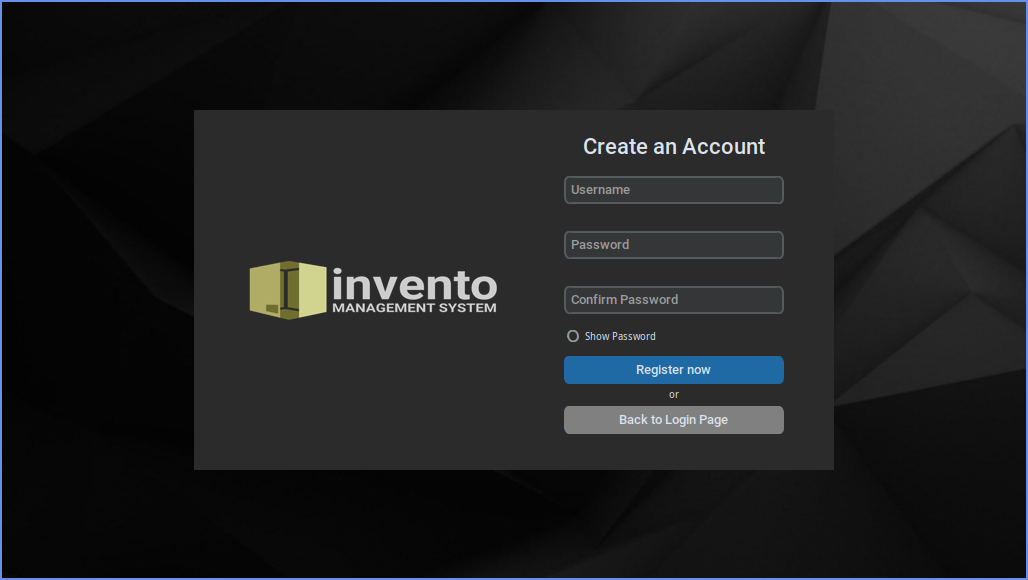
\includegraphics[width=5in,height=3in]{Register.png}
          \caption{Register page}
          \label{fig:register}
        \end{figure}

        To access the inventory management system, log in with a valid username 
        and password. If you do not have an account, Click the "Create an account"
        button on the login page. Once you have created an account, you can log 
        in and begin using the system.

        After logging in, the Dashboard Tab (Figure \ref{fig:dashboard}) is shown. 
        It displays the overall changes done in the inventory and current number of
        users, products, categories, and total sales. 

        \begin{figure}[ht]
          \centering
          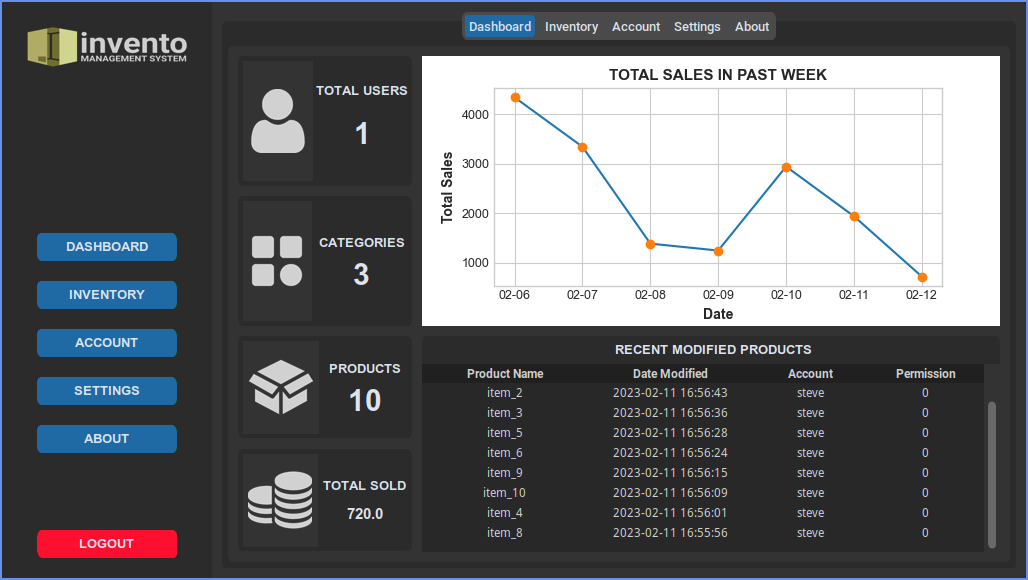
\includegraphics[width=5in,height=3in]{Dashboard.png}
          \caption{Dashboard Tab}
          \label{fig:dashboard}
        \end{figure}

        The Inventory Tab (Figure \ref{fig:inventory}), is where you manage the
        products, categories, and sales, There also is the search functionality that
        enables quickly look up for an item you desire to look into. If you wanted to
        sort the item based on stock, name, data modified, etc., you can click the
        header of the table to trigger it into ascending and descending order.

        \begin{figure}[ht]
          \centering
          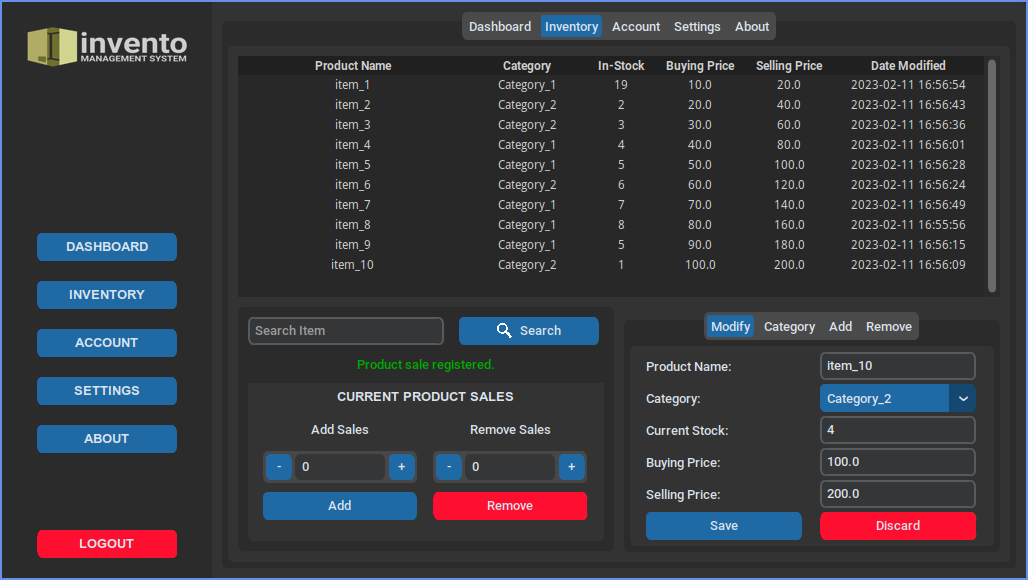
\includegraphics[width=5in,height=3in]{Inventory.png}
          \caption{Inventory Tab}
          \label{fig:inventory}
        \end{figure}

    \newpage

        In this page (Figure \ref{fig:account}), is where you manage your account
        and view other accounts. There are two levels of permission given for an
        account, the \texttt{User Account} and the \texttt{Administrator Account}.
        User accounts can access the normal features given in the program, 
        like the inventory management feature. The latter, administrator account, 
        can access the whole features including account deletion, resetting the
        inventory, and changing permissions for user accounts.

        \begin{figure}[ht]
          \centering
          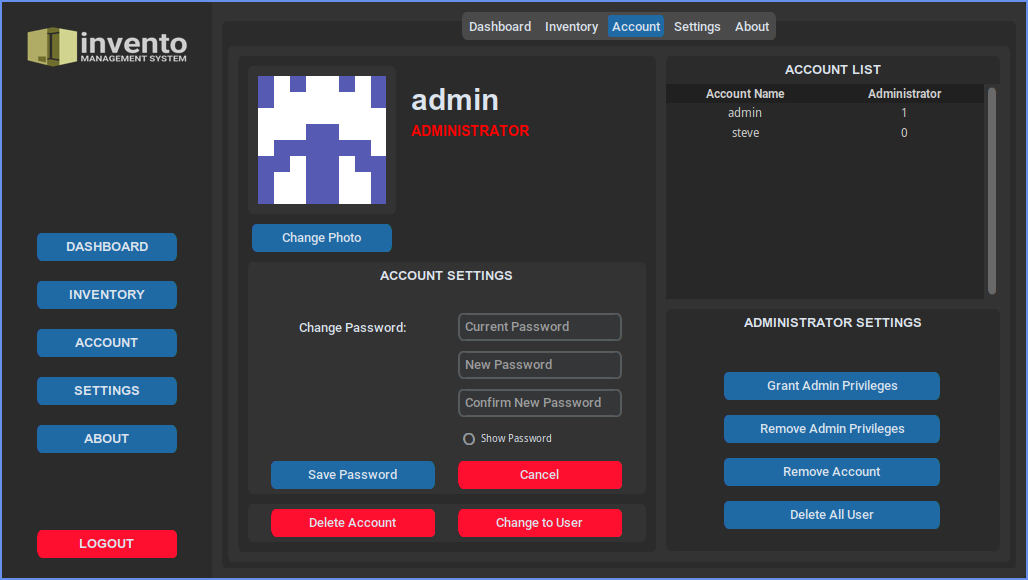
\includegraphics[width=5in,height=3in]{Account.png}
          \caption{Accounts Tab}
          \label{fig:account}
        \end{figure}

        The Settings Tab (Figure \ref{fig:settings}) handles all theme changes 
        and widget scaling. There currently are two appearances, the 
        \texttt{Light} and \texttt{Dark} appearance. The theme can be changed into 
        \texttt{blue}, \texttt{dark-blue}, and \texttt{green}. For the rest, you can 
        find out by trying the program.

        \begin{figure}[ht]
          \centering
          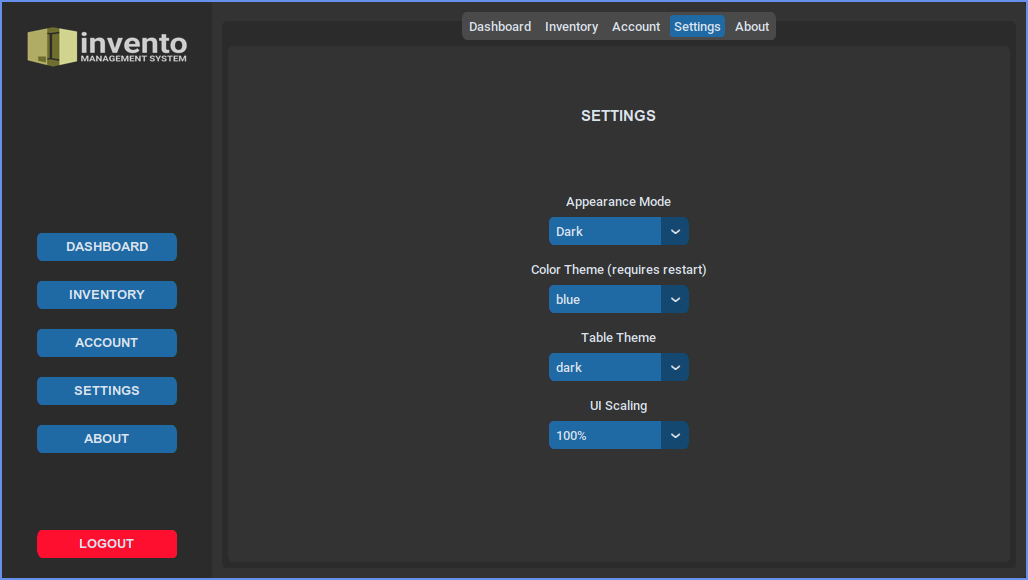
\includegraphics[width=5in,height=3in]{Settings.png}
          \caption{Settings Tab}
          \label{fig:settings}
        \end{figure}


    \newpage
    \part{ Process and Tools }
    
    \indent
    This software is built using modular, object-oriented structure, with focus on 
    readability, maintainability, and extensibility. It follows a traditional 
    Model-View-Controller (MVC) architecture, with separate components managing the 
    user interface, logic, and database interactions.

    \section*{Flowchart}
        \addcontentsline{toc}{section}{Flowchart}
        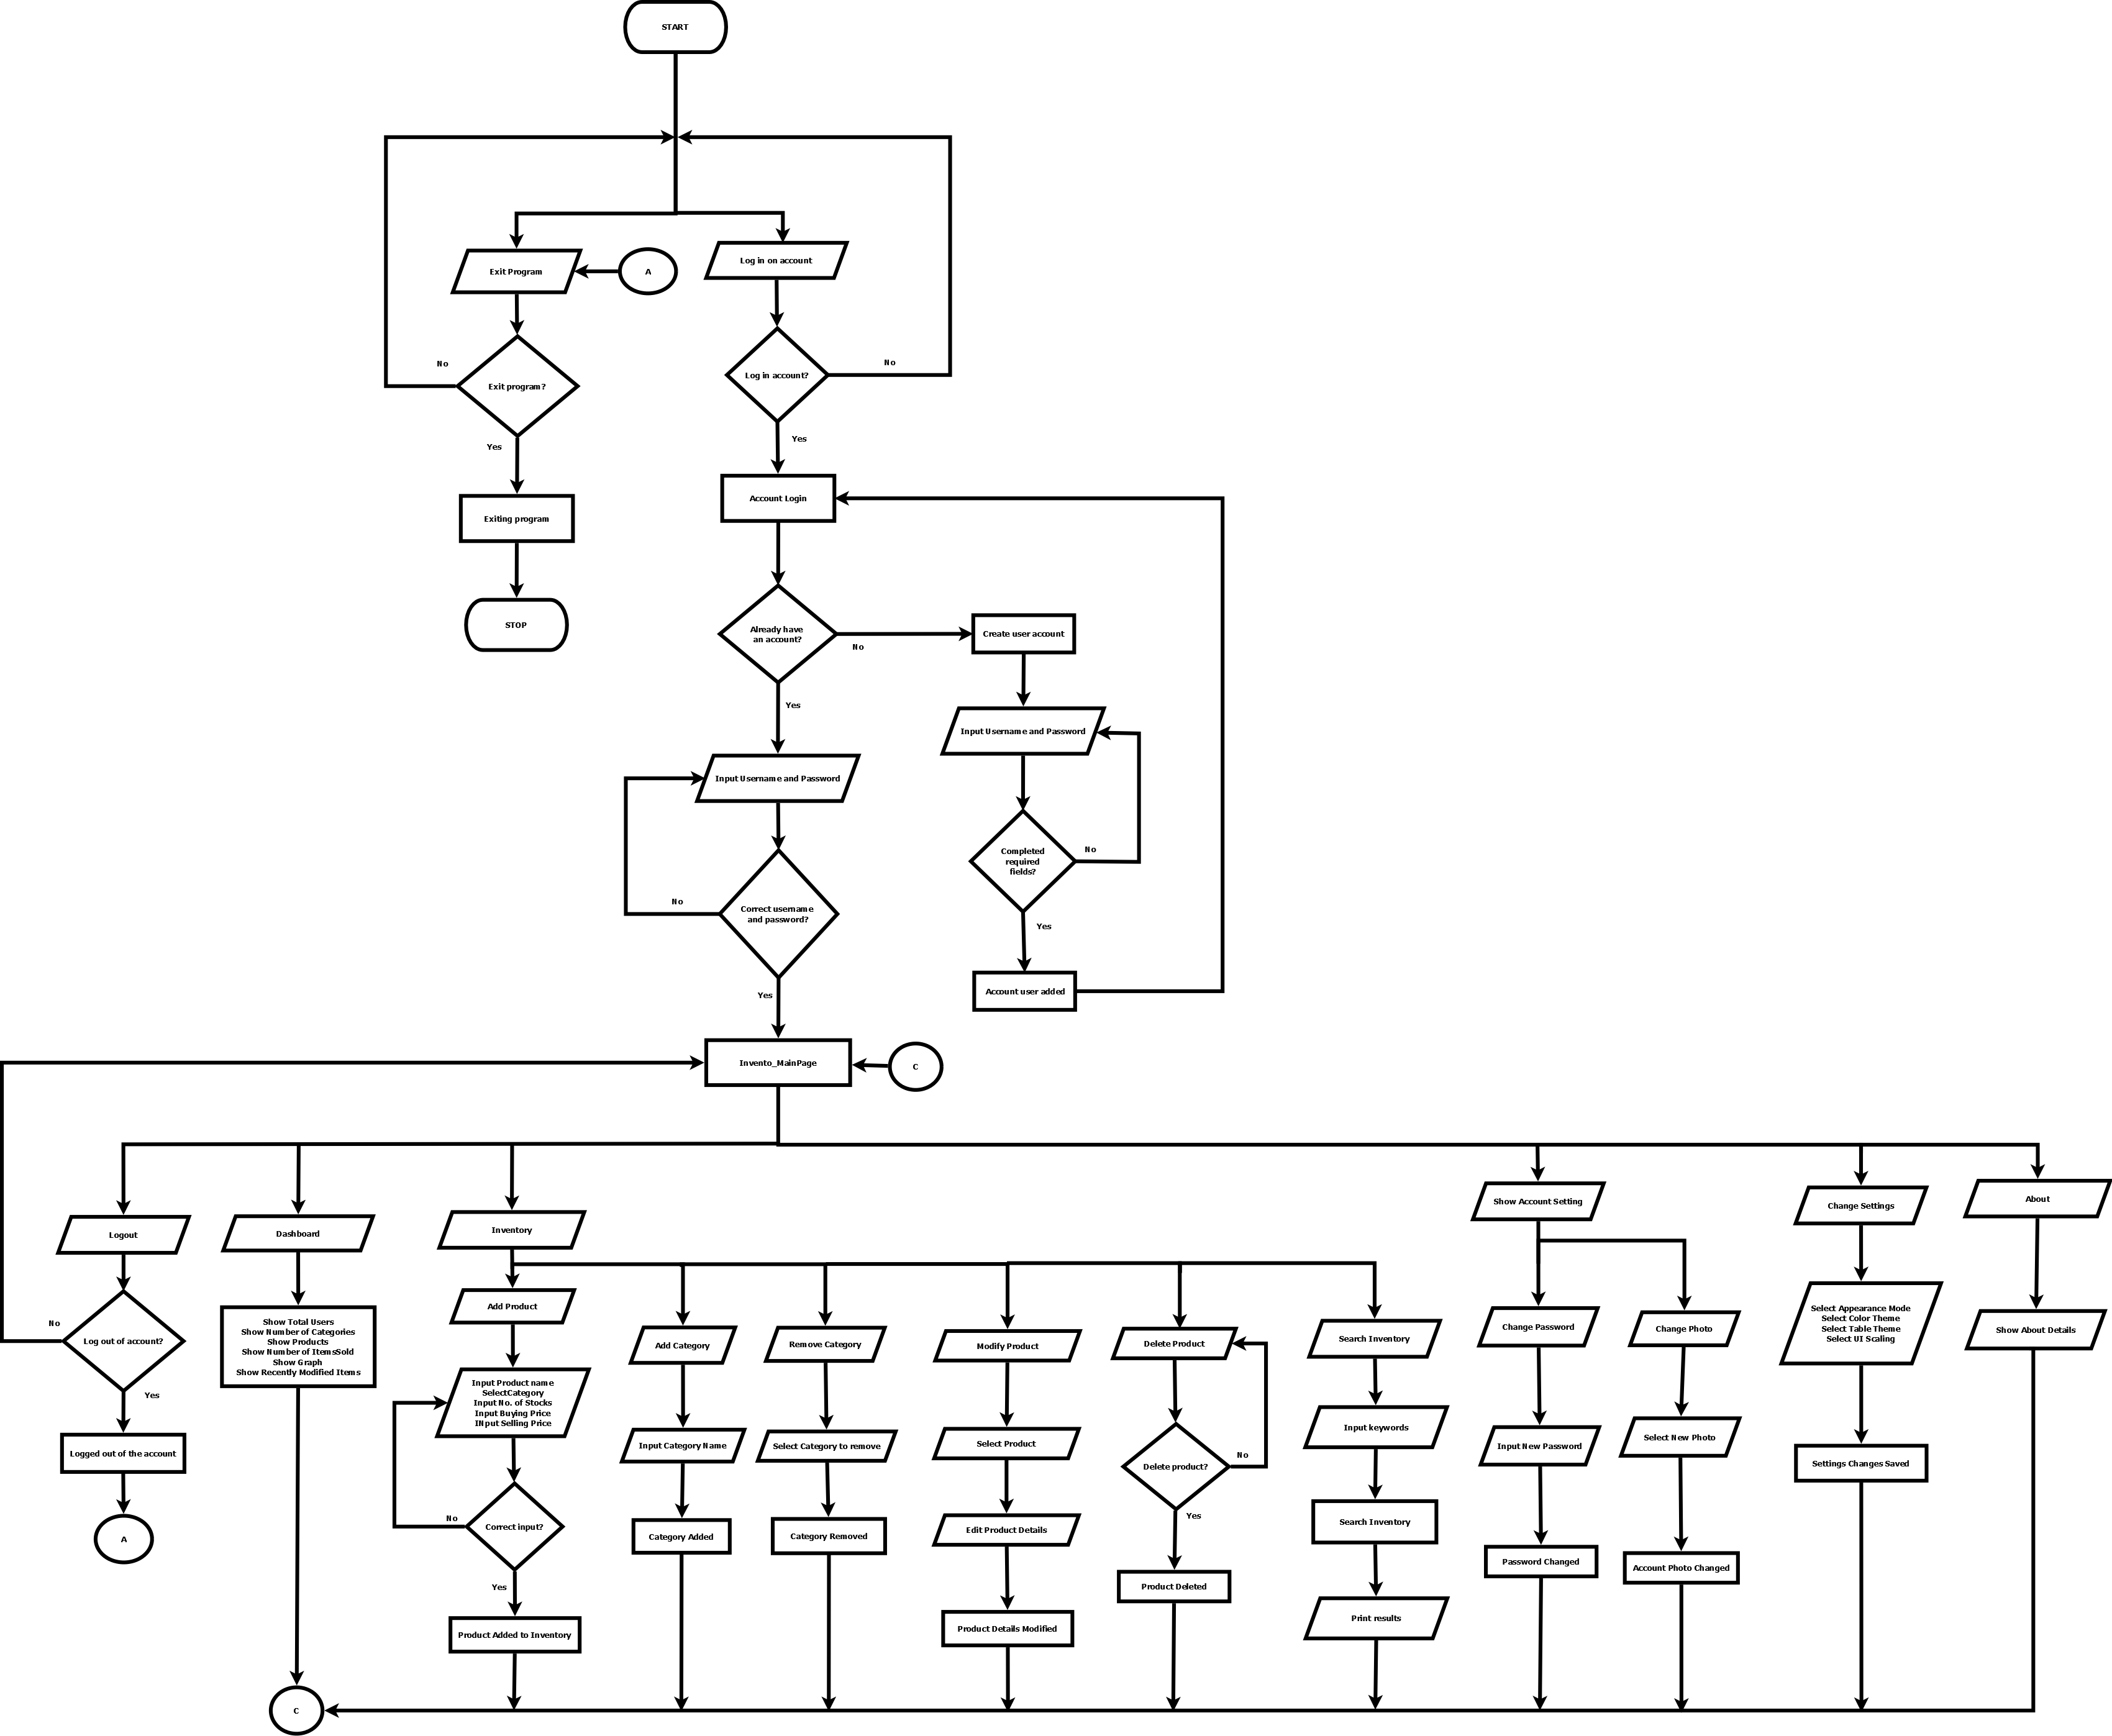
\includegraphics[width=\textwidth,height=5.5in]{Flowchart.png}

    \section*{Database}
        \addcontentsline{toc}{section}{Database}

        \indent
        Invento uses a relational database to store product data, sales data, and 
        account information. The database is managed using the Python \texttt{sqlite} 
        module, which provides a simple and efficient interface for executing SQL 
        queries and managing database connection.

    \section*{User Interface}
        \addcontentsline{toc}{section}{User Interface}

        \indent
        The user interface of this software is implemented using graphical user 
        interface (GUI) framework, such as \texttt{TKinter} and \texttt{Customtkinter}. We aimed for the interface design that is minimal, intuitive and user-friendly, 
        with a clean modern layout.

    \section*{Development Tools}
        \addcontentsline{toc}{section}{Development Tools}

        \indent The following tools are used to develop the program.

        \begin{enumerate}
            \item[\faCode]  \textbf{Programming Language} 
                \begin{enumerate}
                    \item[] \texttt{Python 3.10}
                \end{enumerate}
            \item[\faGears]  \textbf{Frameworks and Libraries} 
                \begin{enumerate}
                    \item[] \texttt{Customtkinter} - GUI framework/package
                    \item[] \texttt{TKinter} - GUI framework
                    \item[] \texttt{Pillow} - image processing
                    \item[] \texttt{Matplotlib} - data visualization
                \end{enumerate}
            \item[\faDatabase]  \textbf{Database and Configurations} 
                \begin{enumerate}
                    \item[] \texttt{SQLite3} - creates \texttt{*.db} file for database
                    \item[] \texttt{Configparser} - creates \texttt{*.ini} file for configurations
                \end{enumerate}
            \item[\faEdit]  \textbf{Text editor or Integrated Development Environment (IDE)} 
                \begin{enumerate}
                    \item[] \texttt{Neovim} - terminal based text editor
                    \item[] \texttt{Pycharm} - IDE
                \end{enumerate}
            \item[\faGithub]  \textbf{Version Control System (VCS)} 
                \begin{enumerate}
                    \item[] \texttt{Git} - local VCS
                    \item[] \texttt{Github} - \href{https://github.com/steguiosaur/invento}{\textcolor{blue}{https://github.com/steguiosaur/invento}}.
                \end{enumerate}
            \item[\faPaintBrush]  \textbf{Creative Tools} 
                \begin{enumerate}
                    \item[] \texttt{GIMP} - photo editor
                    \item[] \texttt{Inkscape} - vector graphics editor; used in logo creation
                    \item[] \texttt{Canva} - used in presentations
                    \item[] \texttt{Figma} - used for structuring GUI in early versions
                    \item[] \texttt{Dia} - flowchart
                \end{enumerate}
            \item[\faFileText]  \textbf{Mark-up Language} 
                \begin{enumerate}
                    \item[] \texttt{Markdown} - README files
                    \item[] \LaTeX{} - used for creating this documentation
                \end{enumerate}
        \end{enumerate}


    \newpage
    \part{ Code Documentation }

    There were several naming conventions used in the code.

    \begin{enumerate}
        \item[] \textbf{Pascal case} is used for \texttt{ClassNames}
        \item[] \textbf{Camel case} is used for \texttt{objectNames}
        \item[] \textbf{Snake case} is used for \texttt{function\_names} and \texttt{method\_names}
    \end{enumerate}

    \section*{Project Structure}
        \addcontentsline{toc}{section}{Project Structure}
    Invento packages and main file.\\
    \begin{forest}
        for tree={font=\sffamily, %grow'=0,
        folder indent=.9em, folder icons,
        edge=densely dotted}
        [\faFolder{} \texttt{invento} 
            [\texttt{customwidget}]
            [\texttt{pages}]
            [\texttt{tabs}]
            [\texttt{utils}]
            [\texttt{Main}, is file]]
    \end{forest}

    \noindent\texttt{customwidget} modules\\
    \begin{forest}
        for tree={font=\sffamily, %grow'=0,
        folder indent=.9em, folder icons,
        edge=densely dotted}
        [\faFolder{} \texttt{customwidget} 
            [\texttt{CtmTreeView}, is file]
            [\texttt{IntSpinBox}, is file]
            [\texttt{LoginBg}, is file]
            [\texttt{SalesGraph}, is file]]
    \end{forest}

    \noindent\texttt{pages} modules\\
    \begin{forest}
        for tree={font=\sffamily, %grow'=0,
        folder indent=.9em, folder icons,
        edge=densely dotted}
        [\faFolder{} \texttt{pages} 
            [\texttt{LoginPage}, is file]
            [\texttt{RegisterPage}, is file]
            [\texttt{InventoryPage}, is file]]
    \end{forest}

    \noindent\texttt{tabs} modules\\
    \begin{forest}
        for tree={font=\sffamily, %grow'=0,
        folder indent=.9em, folder icons,
        edge=densely dotted}
        [\faFolder{} \texttt{tabs} 
            [\texttt{AboutTab}, is file]
            [\texttt{AccountTab}, is file]
            [\texttt{DashboardTab}, is file]
            [\texttt{ProductTab}, is file]
            [\texttt{SettingsTab}, is file]]
    \end{forest}

    \noindent\texttt{utils} modules\\
    \begin{forest}
        for tree={font=\sffamily, %grow'=0,
        folder indent=.9em, folder icons,
        edge=densely dotted}
        [\faFolder{} \texttt{utils} 
            [\texttt{\small accounts}, is file]
            [\texttt{\small assets}, is file]
            [\texttt{\small dependencies}, is file]
            [\texttt{\small icons}, is file]
            [\texttt{\small itemdata}, is file]
            [\texttt{\small randompic}, is file]
            [\texttt{\small settings}, is file]]
    \end{forest}

    \section*{Main file}
        \addcontentsline{toc}{section}{Main file}

        \indent \texttt{Main.py} or the main file, is responsible for executing the app. 
        This can be triggered by using the command \texttt{python Main.py}. It is located at the root of the project with other packages.

    \begin{forest}
        for tree={font=\sffamily, %grow'=0,
        folder indent=.9em, folder icons,
        edge=densely dotted}
        [\faFolder{} \texttt{invento} 
            [\texttt{customwidget}]
            [\texttt{pages}]
            [\texttt{tabs}]
            [\texttt{utils}]
            [\texttt{Main}, is file]]
    \end{forest}

        \subsection*{\normalfont{\faCode{}} \textbf{Main.py}}
            \addcontentsline{toc}{subsection}{Main.py}

        \indent This first part of the code imports several modules from \texttt{utils} package. 
        It calls \texttt{dependency\_installer()} function from \texttt{dependencies} 
        module to automate the installation of packages that are not installed.
        \begin{lstlisting}
from utils import accounts, itemdata, settings, dependencies, Assets
dependencies.dependency_installer() # install dependencies
        \end{lstlisting}

        \hfill{}

        After the installation of required packages, it proceeds to import several 
        other packages. \texttt{Customtkinter} and \texttt{TKinter} are responsible 
        for creating the window where the frames will be placed. The \texttt{pages} 
        package imports all of its module [\texttt{LoginPage, RegisterPage, 
        InventoryPage}] to be added onto the frame dictionary.
        \begin{lstlisting}
from customtkinter import CTkFrame, set_appearance_mode, set_default_color_theme, set_widget_scaling
from tkinter import PhotoImage, Tk
from pages import *

class Main(Tk):
    def __init__(self):
        super().__init__()

        # creates container for frames
        container = CTkFrame(self)
        container.pack(side="top", fill="both", expand=True)
        container.grid_rowconfigure(0, weight=1)
        container.grid_columnconfigure(0, weight=1)

        self.frames = {} # create page dictionary
        for f in [InventoryPage, LoginPage, RegisterPage]:
            page = f.__name__
            frame = f(container, self)
            frame.grid(row=0, column=0, sticky="NSEW")
            self.frames[page] = frame
        \end{lstlisting}

        \hfill{}
        
        In this part, the \texttt{self.get\_session()} will display \texttt{InventoryPage} 
        if there is an account that is currently logged in. If not, it will display 
        \texttt{LoginPage} instead.
        \begin{lstlisting}
        # initialize starting frame
        self.get_session()

    # display selected page on top
    def show_frame(self, page, id=None):
        self.id = id
        self.frames[page].tkraise()

    # current logged in account
    def get_session(self):
        if accounts.get_session() is not None:
            self.show_frame("InventoryPage")
        else:
            self.show_frame("LoginPage")
        \end{lstlisting}

        \newpage
        The comment already explains what it does in this part.
        \begin{lstlisting}
# create database and admin account if not exists
accounts.create_table()
itemdata.create_inventory_table()

# initialize settings and themes
settings.initialize_config()
set_appearance_mode(settings.appearance_read())
set_default_color_theme(settings.theme_read())
set_widget_scaling(settings.int_scale_read())

# start application
app = Main()
app.title("Invento")
app.resizable(True, True)
width = 1024
height = 576
x = (app.winfo_screenwidth()/2) - width/2
y = (app.winfo_screenheight()/2) - height/2
app.geometry('%dx%d+%d+%d' % (width, height, x, y))
app.minsize(1024, 576)
app.iconphoto(True, PhotoImage(file=Assets.asset_path('logo.png')))
app.mainloop()
        \end{lstlisting}


    \section*{utils package}
        \addcontentsline{toc}{section}{utils package}

        \indent This package contains the overall functionality of the program. It 
        includes all modules that handle the database, file paths, generation 
        of image, configurations, and other miscellaneous functions.

    \noindent
    \begin{forest}
        for tree={font=\sffamily, %grow'=0,
        folder indent=.9em, folder icons,
        edge=densely dotted}
        [\faFolder{} \texttt{utils} 
            [\texttt{\small accounts}, is file]
            [\texttt{\small assets}, is file]
            [\texttt{\small dependencies}, is file]
            [\texttt{\small icons}, is file]
            [\texttt{\small itemdata}, is file]
            [\texttt{\small randompic}, is file]
            [\texttt{\small settings}, is file]]
    \end{forest}

        \subsection*{\normalfont{\faCode{}} \textbf{accounts.py}}
            \addcontentsline{toc}{subsection}{accounts.py}

        \indent The \texttt{accounts} module handles all account related 
        functionality. It connects itself to the database file named \texttt{invento.db} 
        and the database table named \texttt{accounts} and \texttt{sessions}. 

        \begin{multicols}{2}
        \begin{center}
            \textbf{accounts}\vspace{5pt}

            \begin{tabular}{| c | c | c |}
                \hline
                \texttt{Username} & \texttt{Password} & \texttt{Admin}\\
                \hline
                admin & hashedpass0e4afc3 & 1\\
                \hline
            \end{tabular}

            \textbf{sessions}\vspace{5pt}

            \begin{tabular}{| c |}
                \hline
                \texttt{Username}\\
                \hline
                admin\\
                \hline
            \end{tabular}
        \end{center}
        \end{multicols}

        \hfill{}

        The following are its functions:
        \begin{enumerate}
            \item[\ding{118}]\texttt{change\_pass(username, passwd, new\_passwd, confirm\_passwd)}

                - Verifies password changes. Used by \texttt{AccountTab} on 
                account settings.

            \item[\ding{118}]\texttt{count\_non\_admin\_accounts()}

                - Used by \texttt{DashboardTab} to display current users.

            \item[\ding{118}]\texttt{create\_table()}

                - Creates table for accounts, login session, and an admin account.

            \item[\ding{118}]\texttt{delete\_all\_users()}

                - Needs admin privileges to delete all users. Accessed by 
                \texttt{AccountTab}.

            \item[\ding{118}]\texttt{delete\_user(username)}

                - Accessed by \texttt{AccountTab} to delete an account.

            \item[\ding{118}]\texttt{get\_all\_accounts()}

                - Displays current accounts in the table.

            \item[\ding{118}]\texttt{get\_permission\_level(username)}

                - Returns 1 if session is an admin account, else 0. Used to verify 
                account permissions.

            \item[\ding{118}]\texttt{get\_session()}

                - Returns the current logged in account.

            \item[\ding{118}]\texttt{grant\_admin\_privilege(username)}

                - Gives a user account admin privileges. Requires an admin account.

            \item[\ding{118}]\texttt{login(username, passwd)}

                - Used by \texttt{LoginPage} to verify username and password.

            \item[\ding{118}]\texttt{logout()}

                - Removes account in session. Changes frame to \texttt{LoginPage}.

            \item[\ding{118}]\texttt{register(username, passwd, confirm\_passwd, admin=False)}

                - Creates a new account in the database.

            \item[\ding{118}]\texttt{remove\_admin\_privilege(username)}

                - Removes admin permission. Accessed by \texttt{AccountTab}.
            
        \end{enumerate}

        \subsection*{\normalfont{\faCode{}} \textbf{assets.py}}
            \addcontentsline{toc}{subsection}{assets.py}

            \indent The \texttt{assets} module locates the location of the 
            \texttt{./assets/} folder in the project. Due to different file pathing 
            between platforms, \texttt{Linux} and \texttt{Windows}, using this 
            module makes it compatible on both operating systems.

            \begin{lstlisting}
from pathlib import Path

class Assets:
    OUTPUT_PATH = Path(__file__).parent
    ASSETS_PATH = OUTPUT_PATH / Path("../assets")

    @staticmethod
    def asset_path(path: str) -> Path:
        return Assets.ASSETS_PATH / Path(path)
            \end{lstlisting}

        \newpage

        \subsection*{\normalfont{\faCode{}} \textbf{dependencies.py}}
            \addcontentsline{toc}{subsection}{dependencies.py}

            \indent This module is responsible for automatically installing the 
            required packages listed on \texttt{requirements.txt}. It creates a
            loop, verifying if the package is installed or not. This script 
            only runs on initial execution of the program. It will be triggered 
            again if the config file \texttt{config.ini} is deleted.

            \begin{lstlisting}
from os.path import isfile
import subprocess
import sys

def install(package):
    subprocess.call([sys.executable, "-m", "pip", "install", package])

def dependency_installer():
    # executes installer on first startup
    if not isfile('./config.ini'):
        with open("requirements.txt") as f:
            dependencies = f.read().splitlines()

        for package in dependencies:
            try:
                __import__(package)
            except ImportError:
                install(package)
            \end{lstlisting}

        \subsection*{\normalfont{\faCode{}} \textbf{icons.py}}
            \addcontentsline{toc}{subsection}{icons.py}

            \begin{center}
                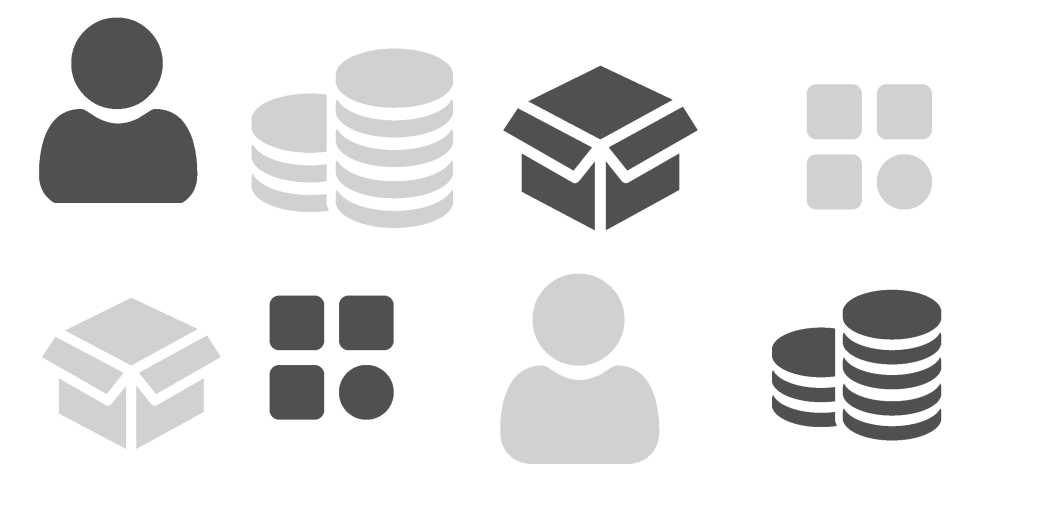
\includegraphics[width=3in,height=1.5in]{iconss.png}
                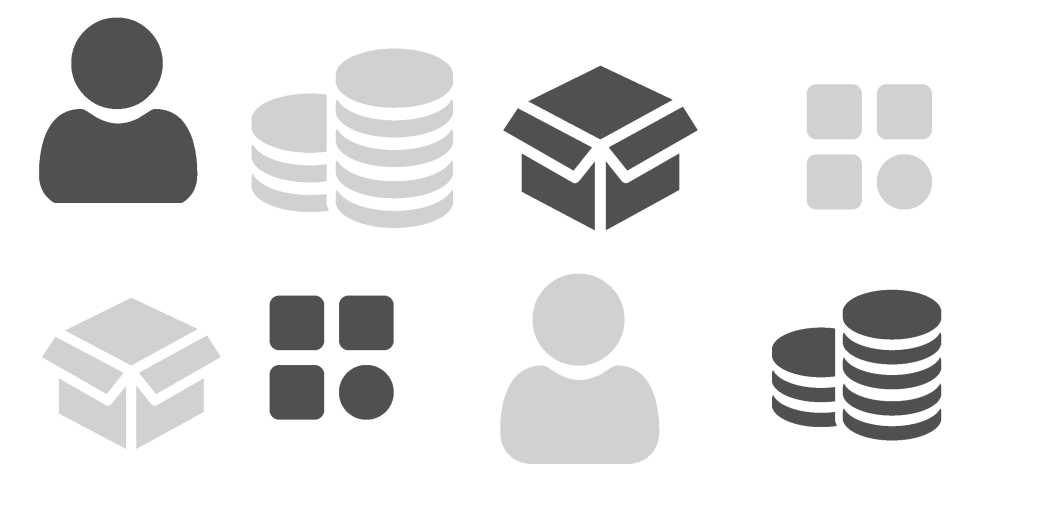
\includegraphics[width=3in,height=1.5in]{iconss.png}
            \end{center}

            \indent The \texttt{icons} module manage the icons being used in 
            \texttt{Dashboard} and \texttt{ProductTab}. It changes according 
            to appearance that was set in the configuration file.


        \subsection*{\normalfont{\faCode{}} \textbf{itemdata.py}}
            \addcontentsline{toc}{subsection}{itemdata.py}

            \indent This module handles all inventory related functionality that 
            accesses the database. It connects on the database file named 
            \texttt{invento.db} and controls three (3) tables named as 
            \texttt{products}, \texttt{categories}, and \texttt{sales}.

        \begin{center}
            \textbf{products}\vspace{5pt}

            \begin{tabular}{| c | c | c | c | c |}
                \hline
                \texttt{items} & \texttt{category} & \texttt{in\_stock} & \texttt{buying\_price} & \texttt{selling\_price}\\
                \hline
                Golden Onion & Spices & 30 & 200.00 & 250.00\\
                \hline
            \end{tabular}

            \begin{tabular}{| c | c | c |}
                \hline
                \texttt{date\_modified} & \texttt{modified\_by} & \texttt{permission\_level}\\
                \hline
                23-02-19 23:43 & admin & 1\\
                \hline
            \end{tabular}

        \end{center}

        \begin{multicols}{2}
        \begin{center}
            \textbf{categories}\vspace{5pt}

            \begin{tabular}{| c |}
                \hline
                \texttt{category\_name}\\
                \hline
                Drinks\\
                \hline
            \end{tabular}

            \textbf{sales}\vspace{5pt}

            \begin{tabular}{| c | c |}
                \hline
                \texttt{total\_sales} & \texttt{date\_sale}\\
                \hline
                11980.00 & 23-02-19\\
                \hline
            \end{tabular}
        \end{center}
        \end{multicols}

        \hfill{}

        \indent The following are its functions:
        \begin{enumerate}
            \item[\ding{118}]\texttt{add\_category(category\_name)}

                - Used in category panel located in \texttt{ProductTab}.

            \item[\ding{118}]\texttt{add\_product(item, category, in\_stock, buying\_price, selling\_price)}

                - Adds the product to inventory table. Used in \texttt{ProductTab}'s 
                add panel.

            \item[\ding{118}]\texttt{add\_sales(earned)}

                - Used by the frame "Current Product Sales" in \texttt{ProductTab}.

            \item[\ding{118}]\texttt{count\_category()}

                - Returns the number of category from the database to be displayed 
                in \texttt{DashboardTab}.

            \item[\ding{118}]\texttt{count\_products()}

                - Returns the number of products from the database to be displayed 
                in \texttt{DashboardTab}.

            \item[\ding{118}]\texttt{create\_inventory\_table()}

                - Responsible for creating the tables named \texttt{accounts}, 
                \texttt{categories}, and \texttt{sales} in the database.

            \item[\ding{118}]\texttt{delete\_all\_products()}

                - Removes all listed products. Requires admin permission.

            \item[\ding{118}]\texttt{delete\_product(product)}

                - Deletes a single selected product. Located at the remove panel in 
                \texttt{ProductTab}.

            \item[\ding{118}]\texttt{edit\_product(product, category, in\_stock, buying\_price, selling\_price, product\_focus)}

                - Updates the product information based on input from modify panel.

            \item[\ding{118}]\texttt{get\_all\_category()}

                - Returns all listed categories from the database to be accessed 
                by the dropdown option menu from \texttt{ProductTab}.

            \item[\ding{118}]\texttt{get\_current\_date\_sales()}

                - Returns the sales of the current date. Unused functionality.

            \item[\ding{118}]\texttt{get\_current\_in\_stock(item\_name)}

                - Reads current number of stock an item have. Used to limit the 
                maximum value of the current stock in adding a sale. Used 
                on "Current Product Sales" panel in \texttt{ProductTab}.

            \item[\ding{118}]\texttt{get\_sales\_data()}

                - Data is used by \texttt{SalesGraph} to be plotted in the line graph 
                at \texttt{DashboardTab}.

            \item[\ding{118}]\texttt{get\_selling\_price(item\_name)}

                - Used by \texttt{add\_sales} and \texttt{remove\_sales} to 
                determine the price of the item.

                add/remove\_sales = number\_of\_product * product\_price

            \item[\ding{118}]\texttt{get\_today\_sales()}

                - Returns the total sales from the database to be displayed 
                in \texttt{DashboardTab}.

            \item[\ding{118}]\texttt{reduce\_sales(remove\_earned)}

                - Used by the frame "Current Product Sales" in \texttt{ProductTab}.

            \item[\ding{118}]\texttt{remove\_category(category\_name)}

                - Removes the selected category in the database's
                \texttt{categories} table.

            \item[\ding{118}]\texttt{search\_product(item\_name)}

                - Used by search entry in \texttt{ProductTab} that filters the entered 
                product to be displayed in the inventory table.

            \item[\ding{118}]\texttt{sort\_table(column, ascending)}

                - Sorts all columns in ascending and descending order. Triggered in 
                the inventory table header.

            \item[\ding{118}]\texttt{update\_stock(item\_name, new\_stock)}

                - Updates the stock after adding or removing a sale.

            \item[\ding{118}]\texttt{view\_inventory()}

                - Displays the inventory table in the \texttt{ProductTab}.

            \item[\ding{118}]\texttt{view\_modified()}

                - Displays the recent modified products table in the 
                \texttt{DashboardTab}.
        \end{enumerate}


        \subsection*{\normalfont{\faCode{}} \textbf{randompic.py}}
            \addcontentsline{toc}{subsection}{randompic.py}

            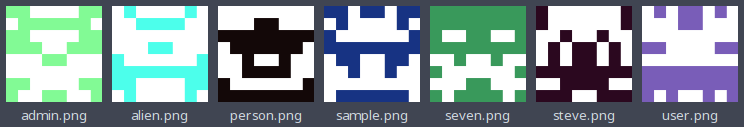
\includegraphics[width=\textwidth,height=1in]{randompics.png}

            This module creates a somewhat high resolution 8x8 pixeled image that is 
            symmetrical in the center x-axis. It acts as a display photo that is 
            different for every account.

            \hfill{}

            In this part of the code, it creates the size, size of pixel boxes, 
            and colors.

            \begin{lstlisting}
    size = (128, 128)
    box_size = size[0] // 8
    white = (255, 255, 255)
    random_color = (random.randint(0, 255), random.randint(0, 255), random.randint(0, 255))
            \end{lstlisting}

            The variable \texttt{random\_color} can generate a total of 16,777,216 
            different RGB color values. This is randomized by the built-in 
            \texttt{random} module of Python.

            $$256 * 256 * 256 = 16777216$$

            In this for loop, it paints the selected box per index with the result 
            from the if-else statement.
            \begin{lstlisting}
    for i in range(4):      # 4 boxes on x-axis
        for j in range(8):  # 8 on y-axis
            if random.choice([True, False]):
                color = random_color
            else:
                color = white
            x1 = i * box_size
            y1 = j * box_size
            x2 = (i + 1) * box_size
            y2 = (j + 1) * box_size
            draw.rectangle([x1, y1, x2, y2], fill=color)
            draw.rectangle([(size[0] - x2), y1, (size[0] - x1), y2], fill=color)
            \end{lstlisting}

            We could calculate the total number of patterns this module
            could generate using this simple permutation formula:

            $$n^{r} = 2^{8 * 4} = 2^{32} = 4294967296$$

            Where $n =$ number of colors, which is \texttt{white} and the 
            \texttt{random\_color}. And $r =$ number of pixels or boxes to be 
            generated with a color. It can generate 4,294,967,296 different patterns without considering the randomization of color value.

            \hfill{} 

            If we try to get the overall randomization with patterns and color value, 
            it reaches an almost incomprehensible total of permutations.

            $$(16777216 + 1 (\normalfont{white}))^{32}$$

            After all the generation of colors and image, it will be stored under 
            the \texttt{./assets/image/} folder.

\begin{lstlisting}
    # store account photo
    path = Path("assets/image") / (username + ".png")
    path.parent.mkdir(parents=True, exist_ok=True)
    image.save(path)
\end{lstlisting}


        \subsection*{\normalfont{\faCode{}} \textbf{settings.py}}
            \addcontentsline{toc}{subsection}{settings.py}

            This module is responsible for reading and writing the preset 
            configuration in the file \texttt{config.ini}.

            \hfill{}

            \faFile{} \textbf{config.ini}
            \begin{lstlisting}
[settings]
appearance = Dark
theme = blue
tablecolor = dark
scale = 100
            \end{lstlisting}

            \begin{figure}[ht]
              \centering
              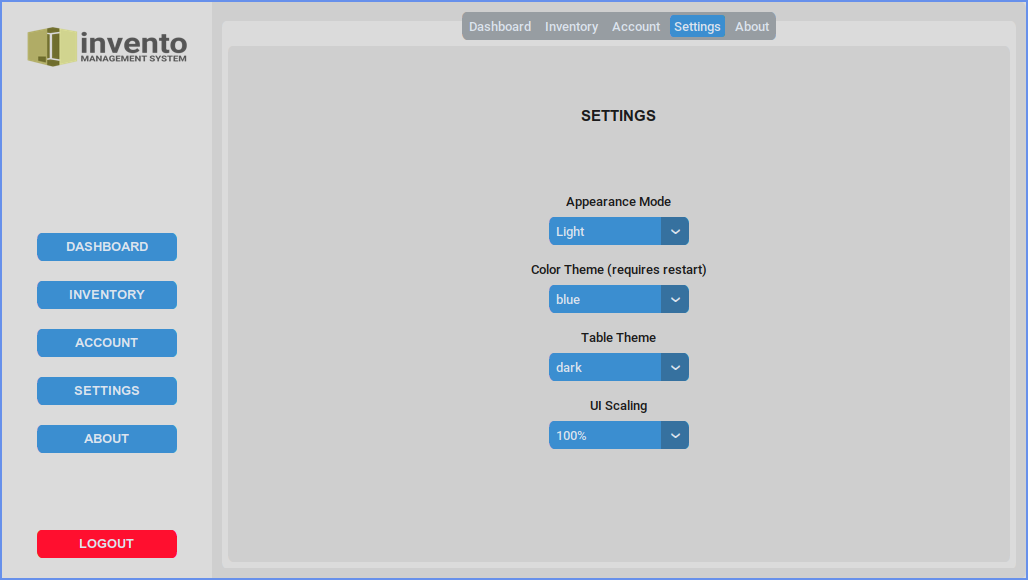
\includegraphics[width=5in,height=3in]{lightsettings.png}
              \caption{Settings Tab}
              \label{fig:lightsettings}
            \end{figure}

            All the backend functionality that Settings Tab does is shown in this code. 
            \begin{lstlisting}
from configparser import ConfigParser
from os.path import isfile

config = ConfigParser()
config.read('config.ini')

# create config at first execute
def initialize_config():
    if not isfile('config.ini'):
        config_set()

# default configuration
def config_set():
    config.add_section('settings')
    config.set('settings', 'appearance', 'Dark')
    config.set('settings', 'theme', 'blue')
    config.set('settings', 'tablecolor', 'dark')
    config.set('settings', 'scale', '100')
    config.write(open('config.ini', 'w'))

# appearance [light, dark]
def appearance_save(appearance):
    config.set('settings', 'appearance', appearance)
    config.write(open('config.ini', 'w'))

# color theme [blue, dark-blue, green]
def theme_save(theme):
    config.set('settings', 'theme', theme)
    config.write(open('config.ini', 'w'))

# table theme [light, dark]
def table_theme_save(table):
    config.set('settings', 'tablecolor', table)
    config.write(open('config.ini', 'w'))

# zoom value [80%, 90%, 100%, 110%, 120%]
def scale_save(scale):
    str_scale = str(int(scale * 100))
    config.set('settings', 'scale', str_scale)
    config.write(open('config.ini', 'w'))
            \end{lstlisting}

            This second half of the code is used to initialize the preset configuration 
            when the program starts. You can see it being called on the \texttt{Main} 
            module. It is also used to view the current configuration that was set.
            \begin{lstlisting}
# get current configuration
def appearance_read():
    return (str(config.get('settings', 'appearance')))

def theme_read():
    return (str(config.get('settings', 'theme')))

def table_theme_read():
    return (str(config.get('settings', 'tablecolor')))

def scale_read():
    return (str(config.get('settings', 'scale'))+"%")

def int_scale_read():
    return int(config.get('settings', 'scale')) /100
            \end{lstlisting}


    \section*{customwidget package}
        \addcontentsline{toc}{section}{customwidget package}

        \indent All modules that can be seen here are mostly customized widgets 
        that displays their own functionality and can be called as objects. It 
        is to be able to place them inside other classes.

        \begin{forest}
            for tree={font=\sffamily, %grow'=0,
            folder indent=.9em, folder icons,
            edge=densely dotted}
            [\faFolder{} \texttt{customwidget} 
                [\texttt{CtmTreeView}, is file]
                [\texttt{IntSpinBox}, is file]
                [\texttt{LoginBg}, is file]
                [\texttt{SalesGraph}, is file]]
        \end{forest}

        \subsection*{\normalfont{\faCode{}} \textbf{CtmTreeView.py}}
            \addcontentsline{toc}{subsection}{CtmTreeView.py}

            \indent Shows the table widget and manages the table style. Used in 
            \texttt{DashboardTab}, \texttt{ProductTab}, and \texttt{AccountTab}.

            \begin{figure}[ht]
              \centering
              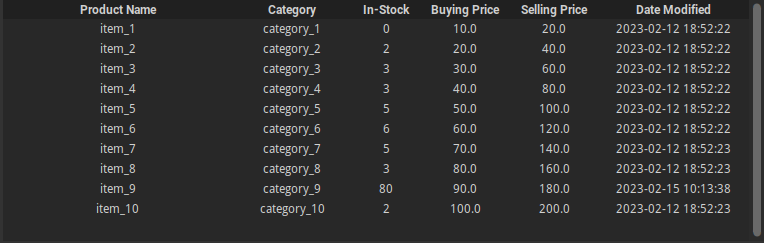
\includegraphics[width=\textwidth,height=1.9in]{inventorytable.png}
              \caption{Inventory Table}
              \label{fig:inventorytable}
            \end{figure}

        \subsection*{\normalfont{\faCode{}} \textbf{IntSpinBox.py}}
            \addcontentsline{toc}{subsection}{IntSpinBox.py}

            \indent Used in \texttt{AccountTab} to input product sales.

            \begin{figure}[ht]
              \centering
              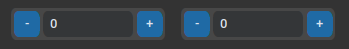
\includegraphics[width=3in,height=.4in]{spinbox.png}
              \caption{SpinBox}
              \label{fig:spinbox}
            \end{figure}

        \subsection*{\normalfont{\faCode{}} \textbf{LoginBg.py}}
            \addcontentsline{toc}{subsection}{LoginBg.py}

            \indent Inherited by \texttt{LoginPage} and \texttt{RegisterPage} 
            to easily manage theme changes. 

            \begin{figure}[ht]
              \centering
              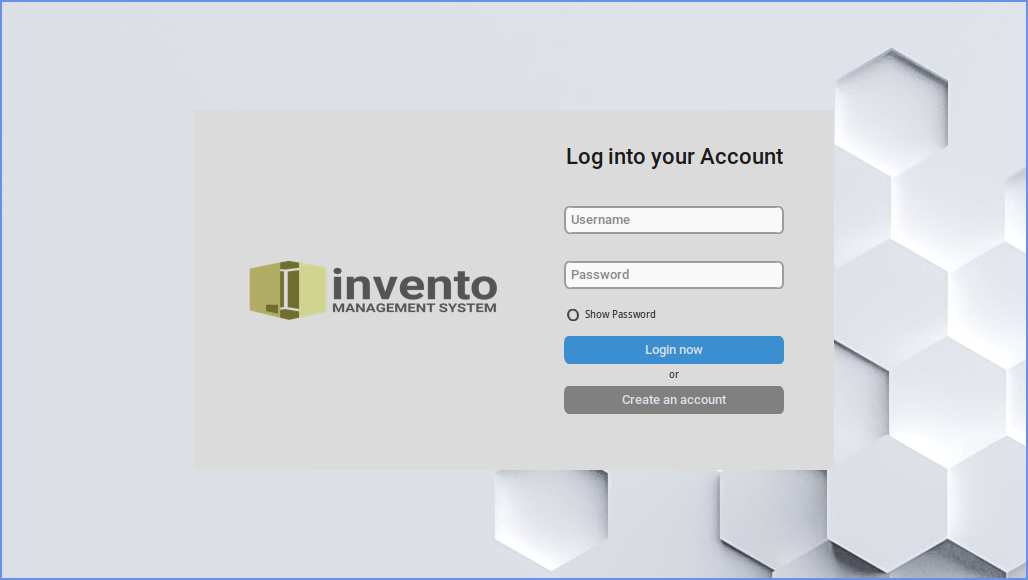
\includegraphics[width=3in,height=1.8in]{lightLogin.png}
              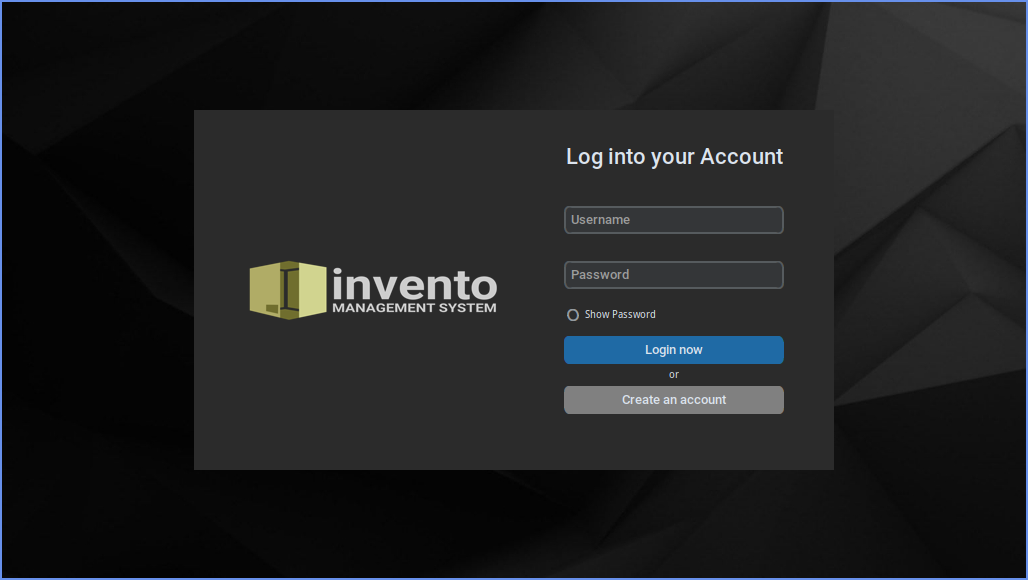
\includegraphics[width=3in,height=1.8in]{Login.png}
              \caption{LoginBg Light and Dark Mode}
              \label{fig:loginbg}
            \end{figure}

        \subsection*{\normalfont{\faCode{}} \textbf{SalesGraph.py}}
            \addcontentsline{toc}{subsection}{SalesGraph.py}

            \indent Displays a line graph and plots the sales per day in 
            \texttt{DashboardTab}. It uses Matplotlib to display the data. 

            \begin{figure}[ht]
              \centering
              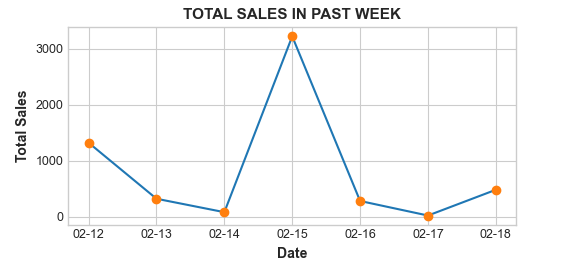
\includegraphics[width=5in,height=2.4in]{salesgraph.png}
              \caption{SalesGraph}
              \label{fig:salesgraph}
            \end{figure}

        \newpage
    
    \section*{Pages}
        \addcontentsline{toc}{section}{Pages}

        \indent The \texttt{pages} package handles all the frames for login, register, 
        and the inventory. The \texttt{Main.py} displays them accordingly to the user's 
        action.

        \begin{forest}
            for tree={font=\sffamily, %grow'=0,
            folder indent=.9em, folder icons,
            edge=densely dotted}
            [\faFolder{} \texttt{pages} 
                [\texttt{LoginPage}, is file]
                [\texttt{RegisterPage}, is file]
                [\texttt{InventoryPage}, is file]]
        \end{forest}

        \subsection*{\normalfont{\faCode{}} \textbf{LoginPage.py}}
            \addcontentsline{toc}{subsection}{LoginPage.py}

            \indent
            The \texttt{LoginPage} module creates an environment inheriting the 
            \texttt{LoginBg} where it allows the user to access the inventory. 
            This also allows the modification of a user, be recorded.

            \begin{center}
              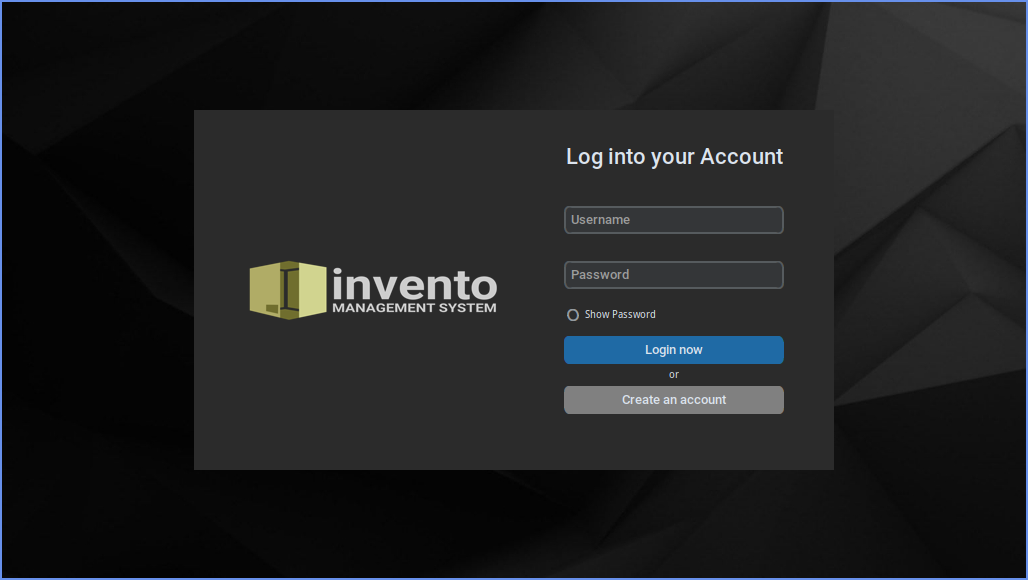
\includegraphics[width=5in,height=3in]{Login.png}
            \end{center}

        \subsection*{\normalfont{\faCode{}} \textbf{RegisterPage.py}}
            \addcontentsline{toc}{subsection}{RegisterPage.py}

            \index This module enables the creation of an account.

            \begin{center}
                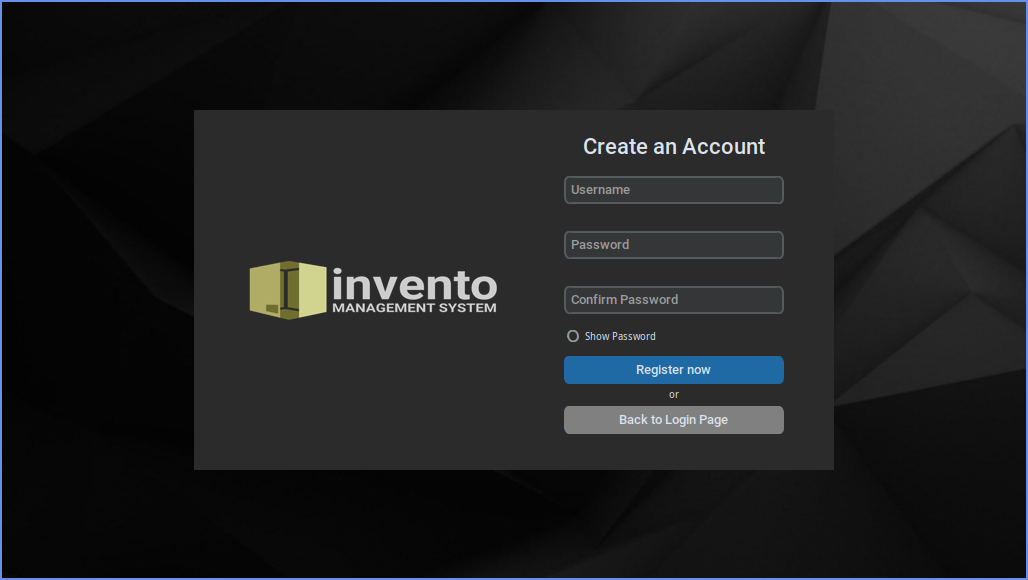
\includegraphics[width=5in,height=3in]{Register.png}
            \end{center}

        \subsection*{\normalfont{\faCode{}} \textbf{InventoryPage.py}}
            \addcontentsline{toc}{subsection}{InventoryPage.py}

            \indent Holds all the tabs, buttons to traverse the tabs, and the 
            logout button.

            \begin{center}
                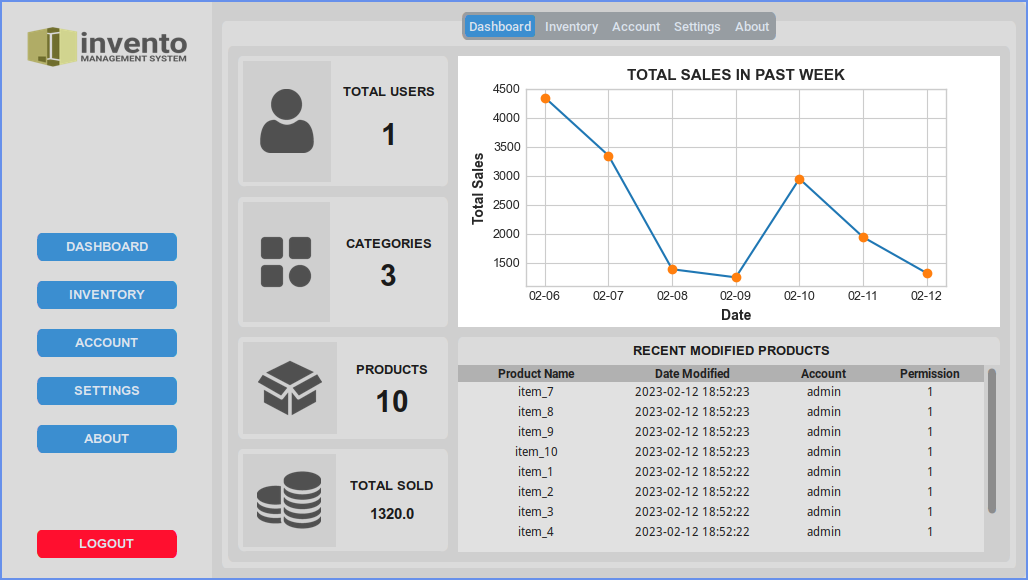
\includegraphics[width=5in,height=3in]{light.png}
            \end{center}

            \begin{lstlisting}
        # DASHBOARD
        self.tabview.tab("Dashboard").grid_columnconfigure(0, weight=1)
        self.tabview.tab("Dashboard").grid_rowconfigure(0, weight=1)
        self.dashboardDisplay = DashboardTab(self.tabview.tab("Dashboard"))
        self.dashboardDisplay.grid(row=0, column=0, sticky="nsew")

        # INVENTORY
        self.tabview.tab("Inventory").grid_columnconfigure(0, weight=1)
        self.tabview.tab("Inventory").grid_rowconfigure(0, weight=1)
        self.inventoryDisplay = ProductTab(self.tabview.tab("Inventory"), controller)
        self.inventoryDisplay.grid(row=0, column=0, sticky="nsew")

        # ACCOUNT
        self.tabview.tab("Account").grid_columnconfigure(0, weight=1)
        self.tabview.tab("Account").grid_rowconfigure(0, weight=1)
        self.accountDisplay = AccountTab(self.tabview.tab("Account"))
        self.accountDisplay.grid(row=0, column=0, sticky="nsew")

        # ABOUTMENU
        self.tabview.tab("About").grid_columnconfigure(0, weight=1)
        self.tabview.tab("About").grid_rowconfigure(0, weight=1)
        self.aboutDisplay = AboutTab(self.tabview.tab("About"))
        self.aboutDisplay.grid(row=0, column=0, sticky="nsew")
        
        # SETTINGS
        self.tabview.tab("Settings").grid_columnconfigure(0, weight=1)
        self.tabview.tab("Settings").grid_rowconfigure(0, weight=1)
        self.settingsDisplay = SettingsTab(self.tabview.tab("Settings"), controller)
        self.settingsDisplay.grid(row=0, column=0, sticky="nsew")
            \end{lstlisting}

            \newpage
    \section*{Tabs}
        \addcontentsline{toc}{section}{Tabs}

        \indent This package contains all the frames for \texttt{InventoryPage}. 
        Every core functionality of this program is accessed in this part. 
        Each tabprovides a different set of features and functionality.

        \begin{forest}
            for tree={font=\sffamily, %grow'=0,
            folder indent=.9em, folder icons,
            edge=densely dotted}
            [\faFolder{} \texttt{tabs} 
                [\texttt{AboutTab}, is file]
                [\texttt{AccountTab}, is file]
                [\texttt{DashboardTab}, is file]
                [\texttt{ProductTab}, is file]
                [\texttt{SettingsTab}, is file]]
        \end{forest}

        \subsection*{\normalfont{\faCode{}} \textbf{AccountTab.py}}
            \addcontentsline{toc}{subsection}{AccountTab.py}

            \indent The \texttt{AccountTab} module provides the functionality for 
            managing accounts. Users can update their password and delete their 
            account. Administrators on the other hand, has more access to modify 
            its own and other user accounts.

            \begin{center}
                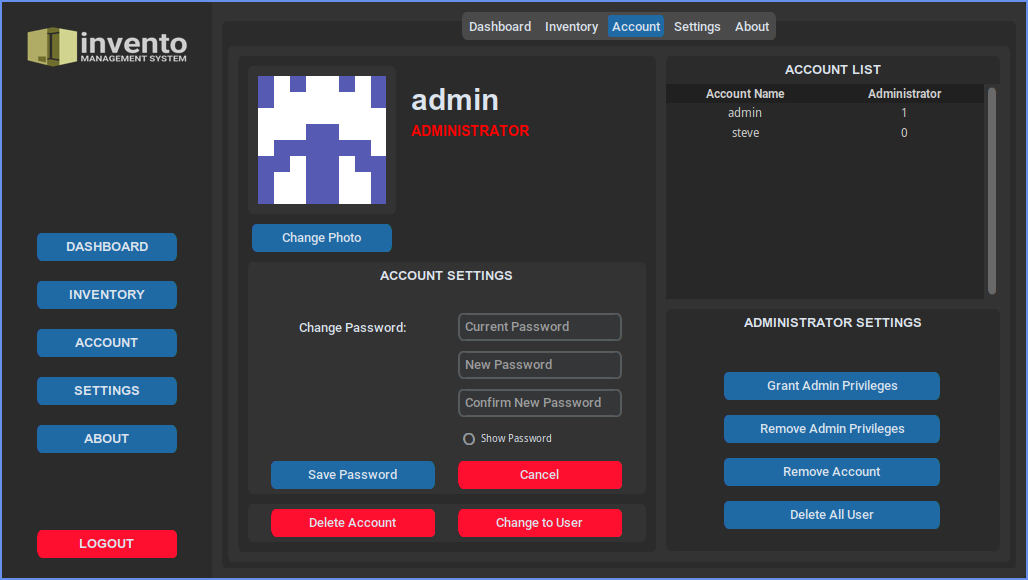
\includegraphics[width=5in,height=2.9in]{Account.png}
            \end{center}

        \subsection*{\normalfont{\faCode{}} \textbf{DashboardTab.py}}
            \addcontentsline{toc}{subsection}{DashboardTab.py}

            \indent The \texttt{DashboardTab} provides an overview of the 
            inventory's modification and sales. 

            \begin{center}
                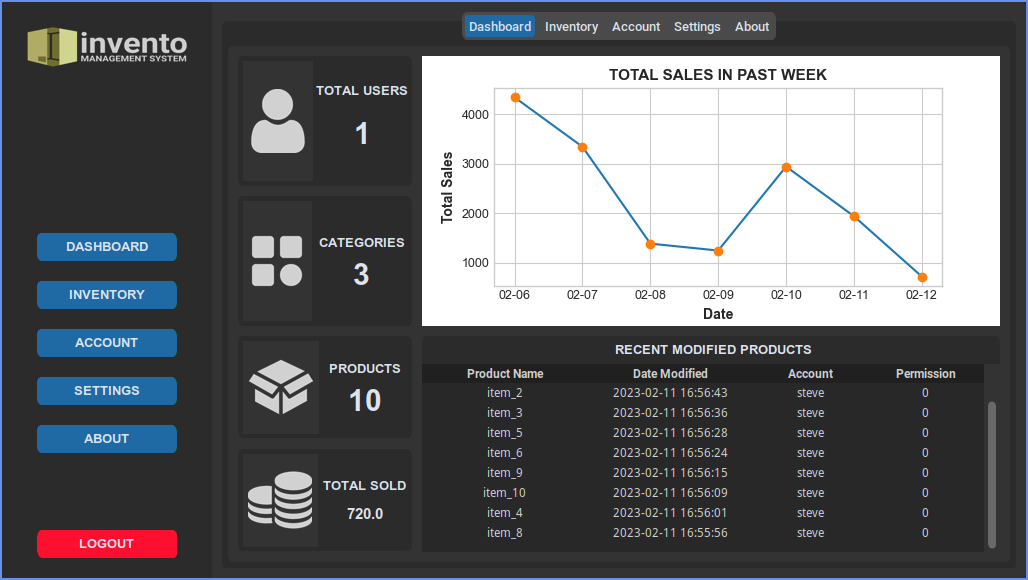
\includegraphics[width=5in,height=2.9in]{Dashboard.png}
            \end{center}

        \subsection*{\normalfont{\faCode{}} \textbf{ProductTab.py}}
            \addcontentsline{toc}{subsection}{ProductTab.py}

            \indent The \texttt{ProductTab} provides the functionality to manage the 
            inventory of the business. Users can basically, add, edit, and delete 
            products in the inventory. It also does track the sales in this part.

            \begin{center}
                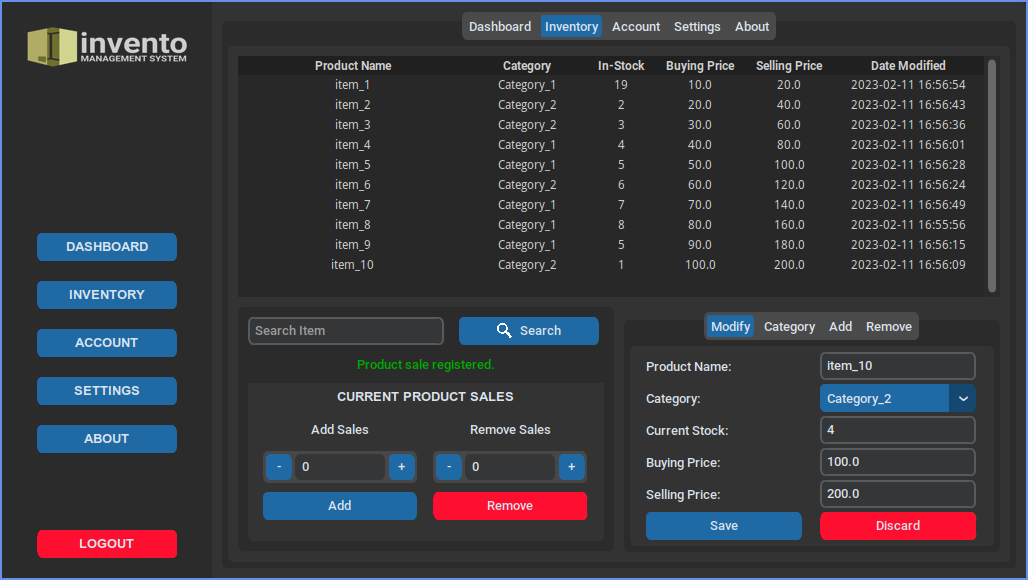
\includegraphics[width=5in,height=2.9in]{Inventory.png}
            \end{center}

        \subsection*{\normalfont{\faCode{}} \textbf{SettingsTab.py}}
            \addcontentsline{toc}{subsection}{SettingsTab.py}

            \indent This part provides options for customizing the application's 
            appearance, theme, and scaling.

            \begin{center}
                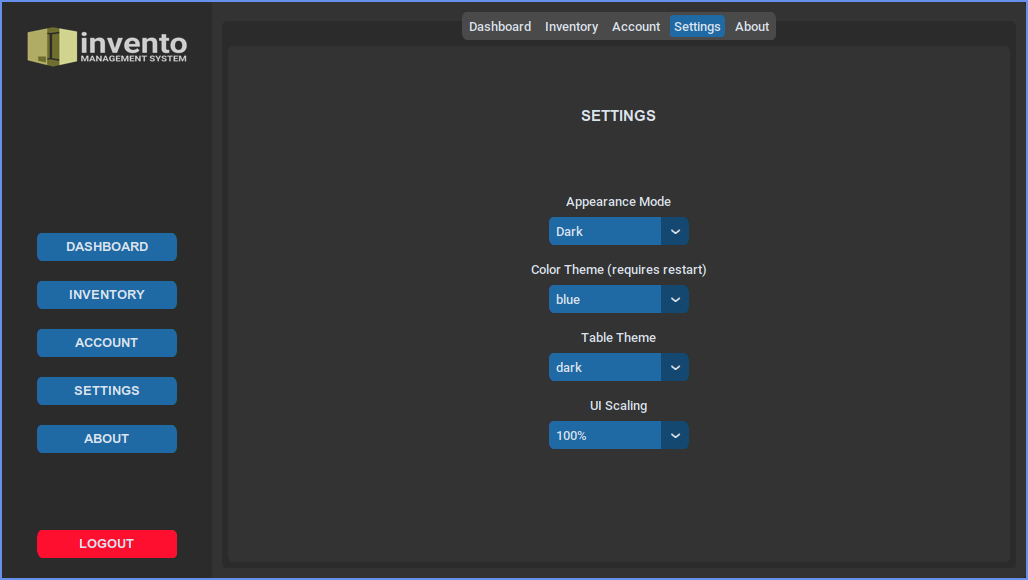
\includegraphics[width=5in,height=2.9in]{Settings.png}
            \end{center}

        \subsection*{\normalfont{\faCode{}} \textbf{AboutTab.py}}
            \addcontentsline{toc}{subsection}{AboutTab.py}

            \indent Shows a short description of the program, the team who created this 
            project, and the core features.

        \hfill{}

        \noindent\dotfill{} END \dotfill

%%%%%%%%%%%%%%%%%%%%%%%%%%%%%%%%%%%% END %%%%%%%%%%%%%%%%%%%%%%%%%%%%%%%%%%%%
\end{document}
%%%%%%%%%%%%%%%%%%%%%%%%%%%%%%%%%%%%%%%%%%%%%%%%%%%%%%%%%%%%%%%%%%%%%%%%%%%%%
